\documentclass[11pt,a4paper]{article}

\usepackage{fontspec}
\setmainfont{Times New Roman}
\setmonofont{Consolas}[Scale=0.95]
\usepackage[a4paper,left=0.8in,right=0.8in,top=0.7in,bottom=0.7in,headheight=14pt,footskip=22pt]{geometry}
\usepackage{graphicx}
\usepackage[export]{adjustbox}
\usepackage{xcolor}
\usepackage{fancyvrb}
\usepackage{fancyhdr}
\usepackage{titlesec}
\usepackage{tocloft}
\usepackage[hidelinks]{hyperref}
\usepackage{microtype}
\usepackage{array}
\usepackage{booktabs}
\usepackage{tabularx}
\usepackage{enumitem}
\usepackage{lastpage}

\definecolor{sqlblue}{HTML}{214F73}
\definecolor{captiongray}{HTML}{444444}
\definecolor{commentgreen}{HTML}{3D6B35}

\pagestyle{fancy}
\fancyhf{}
\fancyfoot[R]{\color{captiongray}\small Бие даалт 10\hspace{1em}\thepage\ / \pageref{LastPage}}
\renewcommand{\headrulewidth}{0pt}
\renewcommand{\footrulewidth}{0pt}

\titleformat{\section}[display]
  {\normalfont\bfseries\color{black}\raggedright}
  {\fontsize{9.5}{11}\selectfont Даалгавар \thesection}
  {1pt}
  {\fontsize{14}{17}\selectfont}
\titlespacing*{\section}{0pt}{0pt}{6pt}

\titleformat{\subsection}{\normalfont\bfseries\fontsize{10.5}{13}\selectfont}{}{0pt}{}
\titlespacing*{\subsection}{0pt}{7pt}{2pt}

\setlength{\parindent}{0pt}
\setlength{\parskip}{4pt}
\setlength{\emergencystretch}{4em}
\renewcommand{\baselinestretch}{1.06}
\setlength{\cftbeforesecskip}{4pt}
\renewcommand{\cftsecfont}{\normalfont}
\renewcommand{\cftsecpagefont}{\normalfont}
\renewcommand{\contentsname}{Агуулга}
\setlist{itemsep=1pt,topsep=2pt}

% Highlighted SQL listings generated by scripts/build_report.py (Pygments).
\input{sql/pygments-style.tex}

% \vshot[max height]{image}{caption}: VS Code SQLTools screenshot. The PNGs are saved at
% 96 DPI, so scale 1.13 prints 0.85pt per pixel and the grid text comes out at body size.
% Tiny results grow to 40% of the text width and wider images shrink to the text width.
% The minipage keeps an image and its caption on one page.
\newcommand{\vshot}[3][0.6\textheight]{%
  \begin{center}\begin{minipage}{\textwidth}\centering
    \includegraphics[scale=1.13,min width=0.4\textwidth,max width=\textwidth,max height=#1]{#2}
    \par\vspace{2pt}
    {\small\color{captiongray}#3\par}
  \end{minipage}\end{center}
}

\newcommand{\id}[1]{\texttt{#1}}
\newcommand{\enquote}[1]{“#1”}

\begin{document}
\sloppy

% ---------------------------------------------------------------------------
\begin{titlepage}
  \thispagestyle{empty}
  \setlength{\parskip}{0pt}
  \centering
  \vspace*{24pt}
  {\bfseries\fontsize{11}{17}\selectfont
    МЭДЭЭЛЛИЙН ТЕХНОЛОГИ,\par
    КОМПЬЮТЕРЫН УХААНЫ ТЭНХИМ\par}

  \vspace{90pt}
  {\bfseries\fontsize{14}{20}\selectfont ӨГӨГДЛИЙН САН\par}
  \vspace{18pt}
  {\bfseries\fontsize{18}{24}\selectfont БИЕ ДААЛТЫН АЖЛЫН ТАЙЛАН\par}
  \vspace{8pt}
  {\fontsize{12}{18}\selectfont Бие даалт № 10\par}
  \vspace{20pt}
  {\fontsize{14}{20}\selectfont Сэдэв: Түр хүснэгт ба хэрэглэгчийн\par
   тодорхойлсон функц (UDF)\par}
  \vspace{6pt}
  {\fontsize{11}{16}\selectfont Northwind өгөгдлийн сан, PostgreSQL 16\par}

  \vspace{60pt}
  {\fontsize{11}{16}\selectfont
    \renewcommand{\arraystretch}{1.5}
    \begin{tabular}{@{}>{\raggedright\arraybackslash}p{1.1in}@{\hspace{14pt}}>{\raggedright\arraybackslash}p{3.55in}@{}}
      Гүйцэтгэсэн: & Дугаржанцан Билгүүн \\
      SISI дугаар: & 23B1NUM1470 \\
      Хөтөлбөр: & Компьютерын ухааны хөтөлбөр
    \end{tabular}\par}

  \vfill
  {\fontsize{11}{16}\selectfont
    Улаанбаатар хот\par
    \vspace{4pt}
    2026 он\par}
  \vspace*{16pt}
\end{titlepage}

\setcounter{page}{2}
\tableofcontents
\thispagestyle{fancy}

% ---------------------------------------------------------------------------
\clearpage
\section*{Ажлын орчин}
\addcontentsline{toc}{section}{Ажлын орчин}

Бүх даалгаврыг Windows 10 дээр суулгасан PostgreSQL 16.15 серверт, Northwind өгөгдлийн сан (91 харилцагч, 830 захиалга, 77 бүтээгдэхүүн, 2155 захиалгын мөр) дээр гүйцэтгэв. Баганын нэрс \id{snake\_case} хэлбэртэй. Бүх код \id{23B1NUM1470\_Дугаржанцан\_Билгүүн\_Биедаалт10.sql} файлд даалгаврын дарааллаар байрлах бөгөөд шинэ холболт дээр эхнээс нь дуустал алдаагүй ажилладаг (\id{psql -v ON\_ERROR\_STOP=1} горимоор шалгасан).

Хэрэглэх зарчим:
\begin{itemize}
  \item Түр хүснэгт бүрийг \id{DROP TABLE IF EXISTS}-ээр эхэлж, хэрэглэж дууссаны дараа мөн \id{DROP TABLE IF EXISTS}-ээр устгасан. Функц доторх түр хүснэгтүүд \id{ON COMMIT DROP} тул дуудлагын transaction дуусахад өөрөө устна.
  \item Функц бүр \id{CREATE OR REPLACE FUNCTION} хэлбэртэй, бүх параметр \id{p\_} угтвартай.
  \item Алдаа гаргах жишээ дуудлагуудыг SQL файлд \id{DO} блок дотор \id{EXCEPTION}-ээр барьж, алдааны мессежийг \id{NOTICE} болгон хэвлэсэн. Ингэснээр скрипт зогсолгүй дуусна. Тайлангийн зурагт эдгээр дуудлагыг шууд ажиллуулж, бодит \id{ERROR} мессежийг харуулав.
  \item Үр дүнгийн зургуудыг VS Code-ийн SQLTools өргөтгөлөөр (\id{Lab 3 Northwind} холболт) асуулга бүрийг ажиллуулж авсан. Зөвхөн CTE хувилбарын бүрэн төлөвлөгөө (Зураг 10.6) нь \id{psql} терминалын гаралт, учир нь SQLTools урт мөрийг тасалдаг.
  \item \id{freight}, \id{unit\_price}, \id{discount} баганууд \id{real} төрөлтэй тул мөнгөн дүнг \id{::numeric} болгож тооцсон. \id{real}-ээс \id{numeric} рүү далд (implicit) хөрвүүлэлт байхгүй тул \id{NUMERIC} параметртэй функцэд \id{freight::numeric} гэж дамжуулна.
\end{itemize}

% ---------------------------------------------------------------------------
\clearpage
\section{Нөөц дуусах дөхсөн бүтээгдэхүүний түр хүснэгт}

\subsection*{Ашигласан арга: түр хүснэгт (\id{CREATE TEMP TABLE ... AS})}
Дутагдалтай бүтээгдэхүүнийг \id{products} хүснэгтээс нэг удаа шүүж \id{low\_stock} түр хүснэгтэд хадгалаад, түүн дээрээ хоёр тайланг ажиллуулсан. Ингэснээр шүүлтийн нөхцөлийг тайлан бүрт давтан бичих шаардлагагүй, түр хүснэгт зөвхөн энэ сешнд харагддаг тул байнгын схемд илүү объект үлдэхгүй. \id{shortage}-ийг \id{reorder\_level - (units\_in\_stock + units\_on\_order)} гэж \id{SELECT} дотор тооцов.

\subsection*{SQL код}
\input{sql/task1.tex}

\subsection*{Үр дүн}
\vshot{img/ss1.png}{Зураг 1.1: Нөхцөлд тэнцсэн 2 бүтээгдэхүүн. Хоёулаа 5 ширхэгээр дутагдалтай.}
\vshot{img/ss2.png}{Зураг 1.2: Beverages, Seafood ангилалд тус бүр 1 дутагдалтай бүтээгдэхүүн байна.}

\subsection*{Асуулт: \id{SELECT * FROM low\_stock;} ажиллуулбал юу болох вэ?}
\id{DROP TABLE}-оос өмнө ижил сешнд ажиллуулбал хүснэгтийн 7 баганатай 2 мөрийг буцаана. Харин ажлын төгсгөлд хүснэгтийг устгасны дараа, эсвэл өөр холболтоос ажиллуулбал \id{ERROR: relation "low\_stock" does not exist} алдаа гарна. Учир нь түр хүснэгт зөвхөн үүсгэсэн сешн дотроо, устгах эсвэл сешн хаагдах хүртэл л оршдог.
\vshot{img/ss27.png}{Зураг 1.3: \id{DROP} хийсний дараах \id{SELECT * FROM low\_stock}.}

% ---------------------------------------------------------------------------
\clearpage
\section{ship\_days() --- хүргэлтийн хоногийг тооцох скаляр функц}

\subsection*{Ашигласан арга: скаляр SQL функц}
Хүргэлтийн хоногийн тооцоо энэ даалгавар болон 6-р даалгаварт давтагддаг тул нэг функц болгосон. Тооцоо нь ганц илэрхийлэл тул \id{LANGUAGE sql} хамгийн энгийн сонголт. PostgreSQL-д \id{date - date} нь хоногийн тоог бүхэл тоогоор буцаадаг. \id{p\_shipped\_date} нь \id{NULL} бол хасах үйлдэл өөрөө \id{NULL} буцаах тул тусгай \id{IF} шалгалт шаардлагагүй.

\subsection*{Яагаад IMMUTABLE вэ?}
Функцийн үр дүн зөвхөн хоёр оролтын огнооноос хамаарна. Хүснэгт уншдаггүй, \id{now()} зэрэг цаг эсвэл тохиргооноос хамаарах функц дууддаггүй тул ижил оролтод үргэлж ижил үр дүн өгнө. Иймд \id{IMMUTABLE} гэж зарласнаар planner функцийг асуулга руу inline хийх, тогтмол аргументтай дуудлагыг урьдчилан тооцох, мөн илэрхийллийн индекст (expression index) ашиглах боломжтой болно.

\subsection*{SQL код}
\input{sql/task2.tex}

\subsection*{Үр дүн}
\vshot{img/ss3.png}{Зураг 2.1: 1997 оны захиалгуудын дундаж хүргэлт 8.9 хоног.}
\vshot{img/ss4.png}{Зураг 2.2: 1997 оны хамгийн удаан хүргэгдсэн 5 захиалга (35--37 хоног).}
\vshot{img/ss5.png}{Зураг 2.3: \id{ship\_days()} нь \id{NULL} буцаасан буюу хүргэгдээгүй 21 захиалга байна.}

% ---------------------------------------------------------------------------
\clearpage
\section{Туршлагатай ажилтнуудын түр хүснэгт}

\subsection*{Ашигласан арга: бүтцийг зарласан түр хүснэгт ба \id{INSERT ... SELECT}}
\id{CREATE TEMP TABLE (...)} хэлбэрээр баганын төрөл болон \id{PRIMARY KEY}-г өөрөө зааж өгсөн тул давхардсан \id{employee\_id} орох боломжгүй, төрөл нь тодорхой. Өгөгдлийг тусад нь \id{INSERT ... SELECT}-ээр оруулснаар хүснэгтийн бүтэц ба өгөгдөл бэлтгэх логик салж, код уншихад ойлгомжтой болсон. \id{full\_name}-ийг \id{||} оператороор залгаж, \id{years\_worked}-ийг \id{EXTRACT(YEAR FROM age(hire\_date))} буюу өнөөдрийг хүртэлх бүтэн жилээр тооцов.

\subsection*{SQL код}
\input{sql/task3.tex}

\subsection*{Үр дүн}
\vshot{img/ss6.png}{Зураг 3.1: 1994-01-01-ээс өмнө ажилд орсон 6 ажилтан. \id{age()} нь өнөөдрийн огноог (2026-10-02) ашигладаг тул ажилласан жил ажиллуулсан өдрөөс хамаарна.}
\vshot{img/ss7.png}{Зураг 3.2: Ажилласан жилийн дундаж 33.2 жил.}

% ---------------------------------------------------------------------------
\clearpage
\section{freight\_class() --- тээврийн зардлын ангилал}

\subsection*{Ашигласан арга: \id{CASE}-тэй скаляр SQL функц}
Ангиллын дүрмийг нэг функцэд тодорхойлсноор \id{GROUP BY} болон \id{WHERE} хоёуланд ижил дүрэм хэрэглэгдэнэ. Хил хязгаар өөрчлөгдвөл зөвхөн функцийг засахад хангалттай. Функц зөвхөн оролтоосоо хамаардаг тул \id{IMMUTABLE}. \id{CASE} нь \id{NULL}-ийг эхэнд шалгаж \id{'Тодорхойгүй'} гэж буцаана, 50--150 (хоёр захаа оролцуулан) нь \id{'Дунд'}.

\subsection*{SQL код}
\input{sql/task4.tex}

\subsection*{Үр дүн}
\vshot{img/ss8.png}{Зураг 4.1: 1997 оны 408 захиалгын ангилал. \id{'Өндөр'} ангилал захиалгын 14\%-ийг эзэлдэг ч нийт freight-ийн 54\%-ийг бүрдүүлж байна. \id{freight} нь \id{NULL} захиалга байхгүй тул \id{'Тодорхойгүй'} мөр гараагүй.}
\vshot{img/ss9.png}{Зураг 4.2: 1997 онд \id{'Өндөр'} ангилалд орсон захиалга хамгийн олонтой 5 улс.}

% ---------------------------------------------------------------------------
\clearpage
\section{Харилцагчийн идэвхийн түр хүснэгт}

\subsection*{Ашигласан арга: түр хүснэгт ба \id{LEFT JOIN}}
Харилцагч бүрийн захиалгын хураангуйг нэг удаа нэгтгэж \id{customer\_activity}-д хадгалаад гурван тайланд дахин ашигласан. Ингэснээр \id{orders} хүснэгтийг гурван удаа \id{GROUP BY} хийх шаардлагагүй болсон. \id{LEFT JOIN} ба \id{COUNT(o.order\_id)} хэрэглэсэн тул захиалгагүй харилцагч \id{orders\_count = 0}-ээр орно (\id{COUNT(*)} бол 1 гэж тоолох байсан). \id{total\_freight}-ийг \id{COALESCE}-ээр 0 болгосон.

\subsection*{SQL код}
\input{sql/task5.tex}

\subsection*{Үр дүн}
Түр хүснэгтэд бүх 91 харилцагч орсон бөгөөд тэдгээрийн 2 нь (FISSA, PARIS) огт захиалга хийгээгүй.
\vshot{img/ss10.png}{Зураг 5.1: (а) Хамгийн олон захиалга хийсэн 10 харилцагч.}
\vshot{img/ss11.png}{Зураг 5.2: (б) 1998 онд захиалга хийгээгүй боловч өмнө нь захиалж байсан 8 харилцагч.}
\vshot{img/ss12.png}{Зураг 5.3: (в) Улс тус бүрийн үзүүлэлт (бүх 21 улс). Франц, Испанид идэвхгүй харилцагч тус бүр 1 байна.}

% ---------------------------------------------------------------------------
\clearpage
\section{shipper\_performance(p\_year) --- хүснэгт буцаадаг функц}

\subsection*{Ашигласан арга: \id{RETURNS TABLE} хэлбэрийн PL/pgSQL функц}
Оноос хамаарсан тайланг функц болгосноор дурын онд дахин ашиглаж, үр дүнг ердийн хүснэгт шиг \id{WHERE}, \id{ORDER BY}-аар боловсруулах боломжтой болсон. Оролтыг шалгаж \id{RAISE EXCEPTION} хийх шаардлагатай тул \id{plpgsql} сонгосон. \id{avg\_ship\_days}-ийг 2-р даалгаврын \id{ship\_days()}-ээр, \id{late\_pct}-ийг \id{NULLIF}-ээр 0-д хуваахаас хамгаалж тооцов. Функц зөвхөн өгөгдөл уншдаг ч хүснэгтийн агуулгаас хамаардаг тул \id{IMMUTABLE} биш, \id{STABLE} байна.

\subsection*{SQL код}
\input{sql/task6.tex}

\subsection*{Үр дүн}
\vshot{img/ss13.png}{Зураг 6.1: Байрлалаар дуудах. 1997 онд United Package хамгийн их хоцролттой (7.2\%).}
\vshot{img/ss14.png}{Зураг 6.2: Нэрээр (\id{=>}) дуудах. 1998 онд Speedy Express (78), Federal Shipping (75) 80-аас цөөн захиалгатай тул \id{HAVING}-ээр хасагдсан.}
\vshot{img/ss15.png}{Зураг 6.3: Үр дүнг \id{WHERE}-ээр шүүх: 1996 онд хоцролт 5\%-иас их тээвэрлэгчид.}
\vshot{img/ss28.png}{Зураг 6.4: \id{SELECT * FROM shipper\_performance(2000)} --- 1996--1998-аас гадуурх он өгөхөд гарах алдаа.}

% ---------------------------------------------------------------------------
\clearpage
\section{pct\_of() функц ба ангиллын орлогын бүтэц}

\subsection*{Ашигласан арга: туслах функц, түр хүснэгт, цонхны функц}
Эзлэх хувийг 0 болон \id{NULL}-ээс хамгаалж тооцох томьёо энэ даалгавар болон 10-р даалгаварт хэрэглэгдэх тул \id{pct\_of()} функц болгосон. 1997 оны ангиллын орлогыг (\id{unit\_price * quantity * (1 - discount)}) нэг удаа нэгтгэж \id{category\_revenue}-д хадгалснаар дараагийн хоёр асуулга 2155 мөрийг дахин нэгтгэхгүй, ердөө 8 мөр дээр ажиллана. Нийт орлогыг \id{SUM(revenue) OVER ()}, хуримтлагдсан дүнг \id{SUM(revenue) OVER (ORDER BY revenue DESC)} цонхны функцээр авсан.

\subsection*{SQL код}
\input{sql/task7.tex}

\subsection*{Үр дүн}
\vshot{img/ss16.png}{Зураг 7.1: 1997 оны ангиллын орлого, эзлэх хувь ба хуримтлагдсан хувь (нийт 617,085.21).}
\vshot{img/ss17.png}{Зураг 7.2: Нийт орлогын 50\%-ийг бүрдүүлэгч ангиллууд.}

Нийт орлогын 50\%-ийг \textbf{Dairy Products, Beverages, Confections, Meat/Poultry} гэсэн 4 ангилал бүрдүүлж байна. Эхний гурав нь хамтдаа 48.9\% буюу 50\%-д арай хүрэхгүй тул Meat/Poultry нэмэгдэж 62.1\% болсноор 50\% давж байна. Асуулга нь өмнөх ангиллуудын хуримтлагдсан хувь (\id{cum\_pct - revenue\_pct}) 50-д хүрээгүй ангиллуудыг сонгодог.

% ---------------------------------------------------------------------------
\clearpage
\section{customer\_rfm() --- функц доторх түр хүснэгт, сегментчлэл}

\subsection*{Ашигласан арга: PL/pgSQL функц доторх \id{ON COMMIT DROP} түр хүснэгт}
RFM шинжилгээ хэд хэдэн алхамтай тул эхний алхмын үр дүнг (recency, frequency, monetary) \id{rfm\_base} түр хүснэгтэд хадгалж, дараагийн алхмуудыг түүн дээр хийсэн. \id{ON COMMIT DROP} нь дуудлагын transaction дуусахад хүснэгтийг автоматаар устгадаг бол эхний \id{DROP TABLE IF EXISTS} нь нэг transaction дотор функцийг дахин дуудахад \enquote{already exists} алдаа гарахаас хамгаална. Оноог \id{UPDATE}-ээр хадгалахын оронд эцсийн \id{SELECT} дотор \id{NTILE(4)}-ээр шууд тооцсон нь хамгийн энгийн арга: нэмэлт хүснэгт ч, \id{UPDATE} ч шаардлагагүй.

Бусад шийдвэр:
\begin{itemize}
  \item Recency бага байх нь сайн тул \id{NTILE(4) OVER (ORDER BY recency\_days DESC)} гэж эрэмбэлсэн: хамгийн удаан захиалаагүй хэсэг 1, хамгийн сүүлд захиалсан хэсэг 4 оноо авна. F, M оноо өсөх эрэмбээр тооцогдоно.
  \item \id{customer\_id} дээр индекс үүсгэж \id{ANALYZE} ажиллуулсан. Autovacuum түр хүснэгтэд статистик цуглуулдаггүй тул \id{ANALYZE}-г гараар хийх шаардлагатай.
  \item Захиалга хийгээгүй 2 харилцагчийн recency тодорхойгүй тул \id{JOIN} ашиглаж тэднийг оруулаагүй (89 харилцагч). Захиалга \id{order\_details}-тэй холбогдсон тул frequency-г \id{COUNT(DISTINCT o.order\_id)}-ээр тоолсон.
\end{itemize}

\subsection*{SQL код}
\input{sql/task8.tex}

\subsection*{Үр дүн}
\vshot{img/ss18.png}{Зураг 8.1: (а) Сегмент тус бүрийн харилцагчийн тоо ба дундаж monetary. Champion сегментийн дундаж худалдан авалт Hibernating-ээс 8 дахин их.}
\vshot{img/ss19.png}{Зураг 8.2: (б) \enquote{At risk} сегментийн monetary-аар эхний 10 харилцагч. Жишээ нь Mère Paillarde 13 захиалга, 28,872.19 дүнтэй ч сүүлийн 188 хоногт захиалга хийгээгүй.}

% ---------------------------------------------------------------------------
\clearpage
\section{restock\_products() --- өгөгдөл өөрчилдөг функц}

\subsection*{Ашигласан арга: өгөгдөл өөрчилдөг PL/pgSQL функц}
Шалгах, шинэчлэх, логлох, алдаа боловсруулах алхмуудыг нэг функцэд нэгтгэснээр бүгд нэг transaction дотор атомаар биелнэ: алдаа гарвал бүх өөрчлөлт буцна. \id{UPDATE ... RETURNING}-ийг \id{WITH changed AS (...) INSERT}-тэй холбосноор шинэчлэлт ба лог нэг statement-ээр бичигддэг. PostgreSQL 16-д \id{RETURNING} зөвхөн шинэ утгыг өгдөг тул \id{products}-ийг өөртэй нь (\id{FROM products AS old}) холбож хуучин утгыг авсан: \id{FROM} хэсгийн мөр өөрчлөлтөөс өмнөх төлөвөөр уншигддаг.

Бусад шийдвэр:
\begin{itemize}
  \item Шинэ утга нь \id{CEIL(reorder\_level * p\_factor)::INT}. Нэмэлт \id{units\_on\_order < CEIL(...)} нөхцөл нь утгыг зөвхөн нэмэгдүүлнэ. Жишээ нь Condiments ангиллын 66-р бүтээгдэхүүний 100 ширхэг захиалга энэ нөхцөлгүй бол 40 болж буурах байсан.
  \item Мөрийн тоог \id{GET DIAGNOSTICS v\_count = ROW\_COUNT}-оор авч, \id{RAISE NOTICE}-ээр хэвлээд буцаана.
  \item Функцийн \id{EXCEPTION WHEN OTHERS} блок ямар ч алдааг барьж, \enquote{restock\_products алдаа: ...} гэсэн ойлгомжтой мессежтэйгээр дахин шиднэ.
  \item Туршилтыг \id{BEGIN ... ROLLBACK} дотор хийсэн тул \id{products}-ийн анхны утга сэргэж, скриптийг дахин ажиллуулахад ижил үр дүн гарна.
\end{itemize}

\subsection*{SQL код}
\input{sql/task9.tex}

\subsection*{Үр дүн}
\vshot{img/ss20.png}{Зураг 9.1: Амжилттай дуудлага. Beverages ангиллын 2 бүтээгдэхүүн шинэчлэгдсэн. Зогсоосон Chang (\id{discontinued = 1}) хамрагдаагүй.}
\vshot{img/ss29.png}{Зураг 9.2: \id{SELECT restock\_products('Beverages', 0.5)} --- \id{p\_factor = 0.5} үед гарах алдаа.}
\vshot{img/ss30.png}{Зураг 9.3: \id{SELECT restock\_products('Electronics')} --- байхгүй ангилал өгөхөд гарах алдаа.}
\vshot{img/ss21.png}{Зураг 9.4: Дуудлагын дараах \id{restock\_log}: Ipoh Coffee 10 \textrightarrow{} 50, Outback Lager 10 \textrightarrow{} 60 (\id{reorder\_level} × 2).}

\subsection*{SQL Server-ийн UDF-д яагаад боломжгүй вэ?}
SQL Server функцийг \id{SELECT} дотор мөр бүрт хэдэн ч удаа, ямар ч дарааллаар дуудаж болох \enquote{цэвэр} илэрхийлэл гэж үздэг тул UDF-д гаж нөлөө (side effect) хориотой. UDF дотор байнгын хүснэгтэд \id{INSERT/UPDATE/DELETE} хийх, \id{\#temp} хүснэгт үүсгэх, \id{TRY...CATCH}, \id{THROW/RAISERROR}, динамик SQL (\id{EXEC}) болон transaction удирдах боломжгүй. Зөвхөн функцийн локал \id{@table} хувьсагчийг өөрчилж болно. Харин PostgreSQL-д \id{VOLATILE} функц өгөгдөл өөрчилж, түр хүснэгт үүсгэж, \id{EXCEPTION} блок ашиглаж чадна.

\subsection*{Функц уу, процедур уу?}
Миний бодлоор энэ үйлдэлд \id{PROCEDURE} (\id{CALL restock\_products(...)}) илүү тохиромжтой. Энэ нь утга тооцдог бус өгөгдөл өөрчилдөг, ганцаараа дуудагддаг үйлдэл бөгөөд процедур нь \id{SELECT} дотор санамсаргүй дуудагдахгүй, дотроо \id{COMMIT/ROLLBACK} хийж transaction-ийг удирдаж чадна. Шинэчилсэн мөрийн тоог \id{INOUT} параметрээр буцааж болно. Харин үр дүнг \id{SELECT}-д шууд ашиглах, бусад асуулгатай нийлүүлэх шаардлагатай бол функц давуу.

% ---------------------------------------------------------------------------
\clearpage
\section{abc\_analysis() --- Парето шинжилгээ ба гүйцэтгэлийн харьцуулалт}

\subsection*{Ашигласан арга: түр хүснэгттэй функц ба зөвхөн CTE-тэй функц}
\id{abc\_analysis()} нь тухайн жилийн бүтээгдэхүүн бүрийн орлогыг \id{product\_revenue} түр хүснэгтэд (\id{ON COMMIT DROP}) хадгалаад, эзлэх хувь, хуримтлагдсан хувь (\id{ROWS UNBOUNDED PRECEDING}) болон A/B/C ангиллыг тооцно. 7-р даалгаврын \id{pct\_of()}-ийг дахин ашигласан. \id{abc\_analysis\_cte()} нь ижил логикийг түр хүснэгтгүй, хоёр CTE-тэй нэг \id{LANGUAGE sql} асуулгаар бичсэн хувилбар. Хоёр хувилбарын үр дүнг \id{EXCEPT}-ээр харьцуулахад 0 мөр гарсан тул үр дүн нь ижил.

\subsection*{SQL код}
\input{sql/task10.tex}

\subsection*{Үр дүн}
\vshot{img/ss22.png}{Зураг 10.1: (а) A/B/C бүлгүүд. 77 бүтээгдэхүүний 36 нь (47\%) 1997 оны орлогын 80\%-ийг бүрдүүлж байна.}
\vshot{img/ss23.png}{Зураг 10.2: (б) A бүлгийн бүтээгдэхүүнүүд ангиллаар. \textbf{Dairy Products} нь A бүлгийн 8 бүтээгдэхүүн, 111,932.84 орлоготой хамгийн чухал ангилал.}
\vshot{img/ss24.png}{Зураг 10.3: Хоёр хувилбарын үр дүнгийн ялгаа 0 мөр.}

\subsection*{EXPLAIN (ANALYZE, BUFFERS) харьцуулалт}
\vshot{img/ss25.png}{Зураг 10.4: Түр хүснэгттэй хувилбарын төлөвлөгөө. PL/pgSQL функц ганц \id{Function Scan} зангилаа болж харагдана.}
\vshot[0.8\textheight]{img/ss26.png}{Зураг 10.5: CTE хувилбарын төлөвлөгөө (SQLTools). Урт мөрүүд тасарч, төлөвлөгөөний эхний хэсэг харагдана.}

Хугацааг тогтвортой болгохын тулд нэг сешнд хувилбар бүрийг ээлжлэн 12 удаа ажиллуулсан. Эхний дуудлагыг тусад нь, үлдсэн 11-ийг медианаар харуулав. Түр хүснэгттэй функцийн дотоод алхмуудын хугацааг \id{auto\_explain} (\id{log\_nested\_statements}) модулиар хэмжсэн.

\begin{center}
\small
\renewcommand{\arraystretch}{1.25}
\begin{tabularx}{\textwidth}{@{}>{\raggedright\arraybackslash}p{1.75in}>{\raggedright\arraybackslash}X>{\raggedright\arraybackslash}X@{}}
\toprule
Үзүүлэлт & Түр хүснэгттэй (\id{abc\_analysis}) & Зөвхөн CTE (\id{abc\_analysis\_cte}) \\
\midrule
Execution Time, эхний дуудлага & 10.59 ms (PL/pgSQL эмхэтгэл орсон) & 2.52 ms \\
Execution Time, медиан (11 удаа) & 3.78 ms (3.75--5.02) & 2.51 ms (2.47--2.57) \\
Planning Time, медиан & 0.01 ms & 0.36 ms \\
Нийт (planning + execution) & $\approx$ 3.79 ms & $\approx$ 2.87 ms \\
Buffers & shared hit $\approx$ 3650, shared dirtied/written 1, local hit/dirtied/written 1 & shared hit 3361, бичилт байхгүй \\
EXPLAIN-д харагдах төлөвлөгөө & Ганц \id{Function Scan}, мөрийн тоог 1000 гэж таамагласан (бодит 77) & Бүрэн төлөвлөгөө: orders \id{Seq Scan} \textrightarrow{} order\_details \id{Bitmap Heap Scan} \textrightarrow{} products \id{Index Scan} \textrightarrow{} categories \id{Hash Join} \textrightarrow{} \id{GroupAggregate} \textrightarrow{} \id{Sort} \textrightarrow{} 2 × \id{WindowAgg} \\
Дотоод алхмууд & \id{CREATE TEMP TABLE AS} $\approx$ 3.4 ms, эцсийн \id{SELECT} $\approx$ 0.13 ms (статистикгүй түр хүснэгтэд 630 мөр гэж таамагласан, бодит 77) & Нэг асуулга. Функц inline хийгдэж, гадна асуулгатай хамт төлөвлөгдсөн \\
\bottomrule
\end{tabularx}
\end{center}

Хоёр хувилбарын холболт (join), нэгтгэлийн төлөвлөгөө адилхан. Ялгаа нь түр хүснэгттэй хувилбар хүснэгт үүсгэх, системийн каталогт бичих, устгах нэмэлт ажил хийдэгт оршино. SQLTools урт мөрийг таслан харуулдаг тул CTE хувилбарын бүрэн төлөвлөгөөг Зураг 10.6-д \id{psql}-ээр үзүүлэв.

\subsection*{Дүгнэлт}
Энэ тохиолдолд CTE хувилбар илүү тохиромжтой. Өгөгдөл бага (77 бүтээгдэхүүн, 1059 захиалгын мөр) бөгөөд завсрын үр дүнг ганц удаа ашигладаг тул түр хүснэгт үүсгэж, каталогт бичиж, устгах зардал (ойролцоогоор 1 ms) нь ашгаасаа их байна. Хэмжилтээр CTE хувилбар ойролцоогоор 2.9 ms, түр хүснэгттэй хувилбар 3.8 ms, эхний дуудлагад PL/pgSQL эмхэтгэл нэмэгдэж 10.6 ms болсон. Мөн \id{LANGUAGE sql} функц асуулга руу inline хийгддэг тул planner бүх төлөвлөгөөг харж оновчилдог бол PL/pgSQL функц planner-ийн хувьд \enquote{хар хайрцаг} (\id{Function Scan}, 1000 мөр гэсэн таамаг) болдог. Харин завсрын үр дүн том бөгөөд олон асуулгад дахин ашиглагддаг, түүн дээр индекс үүсгэх шаардлагатай, эсвэл CTE-ийн мөрийн тооцоолол буруу байж төлөвлөгөө муу гардаг үед \id{ANALYZE} хийсэн түр хүснэгт planner-д бодит статистик өгч илүү хурдан ажиллана. Мөн алхам бүрийн үр дүнг шалгах шаардлагатай, олон алхамтай урт боловсруулалтад түр хүснэгт илүү ойлгомжтой.

\clearpage
\begin{center}
  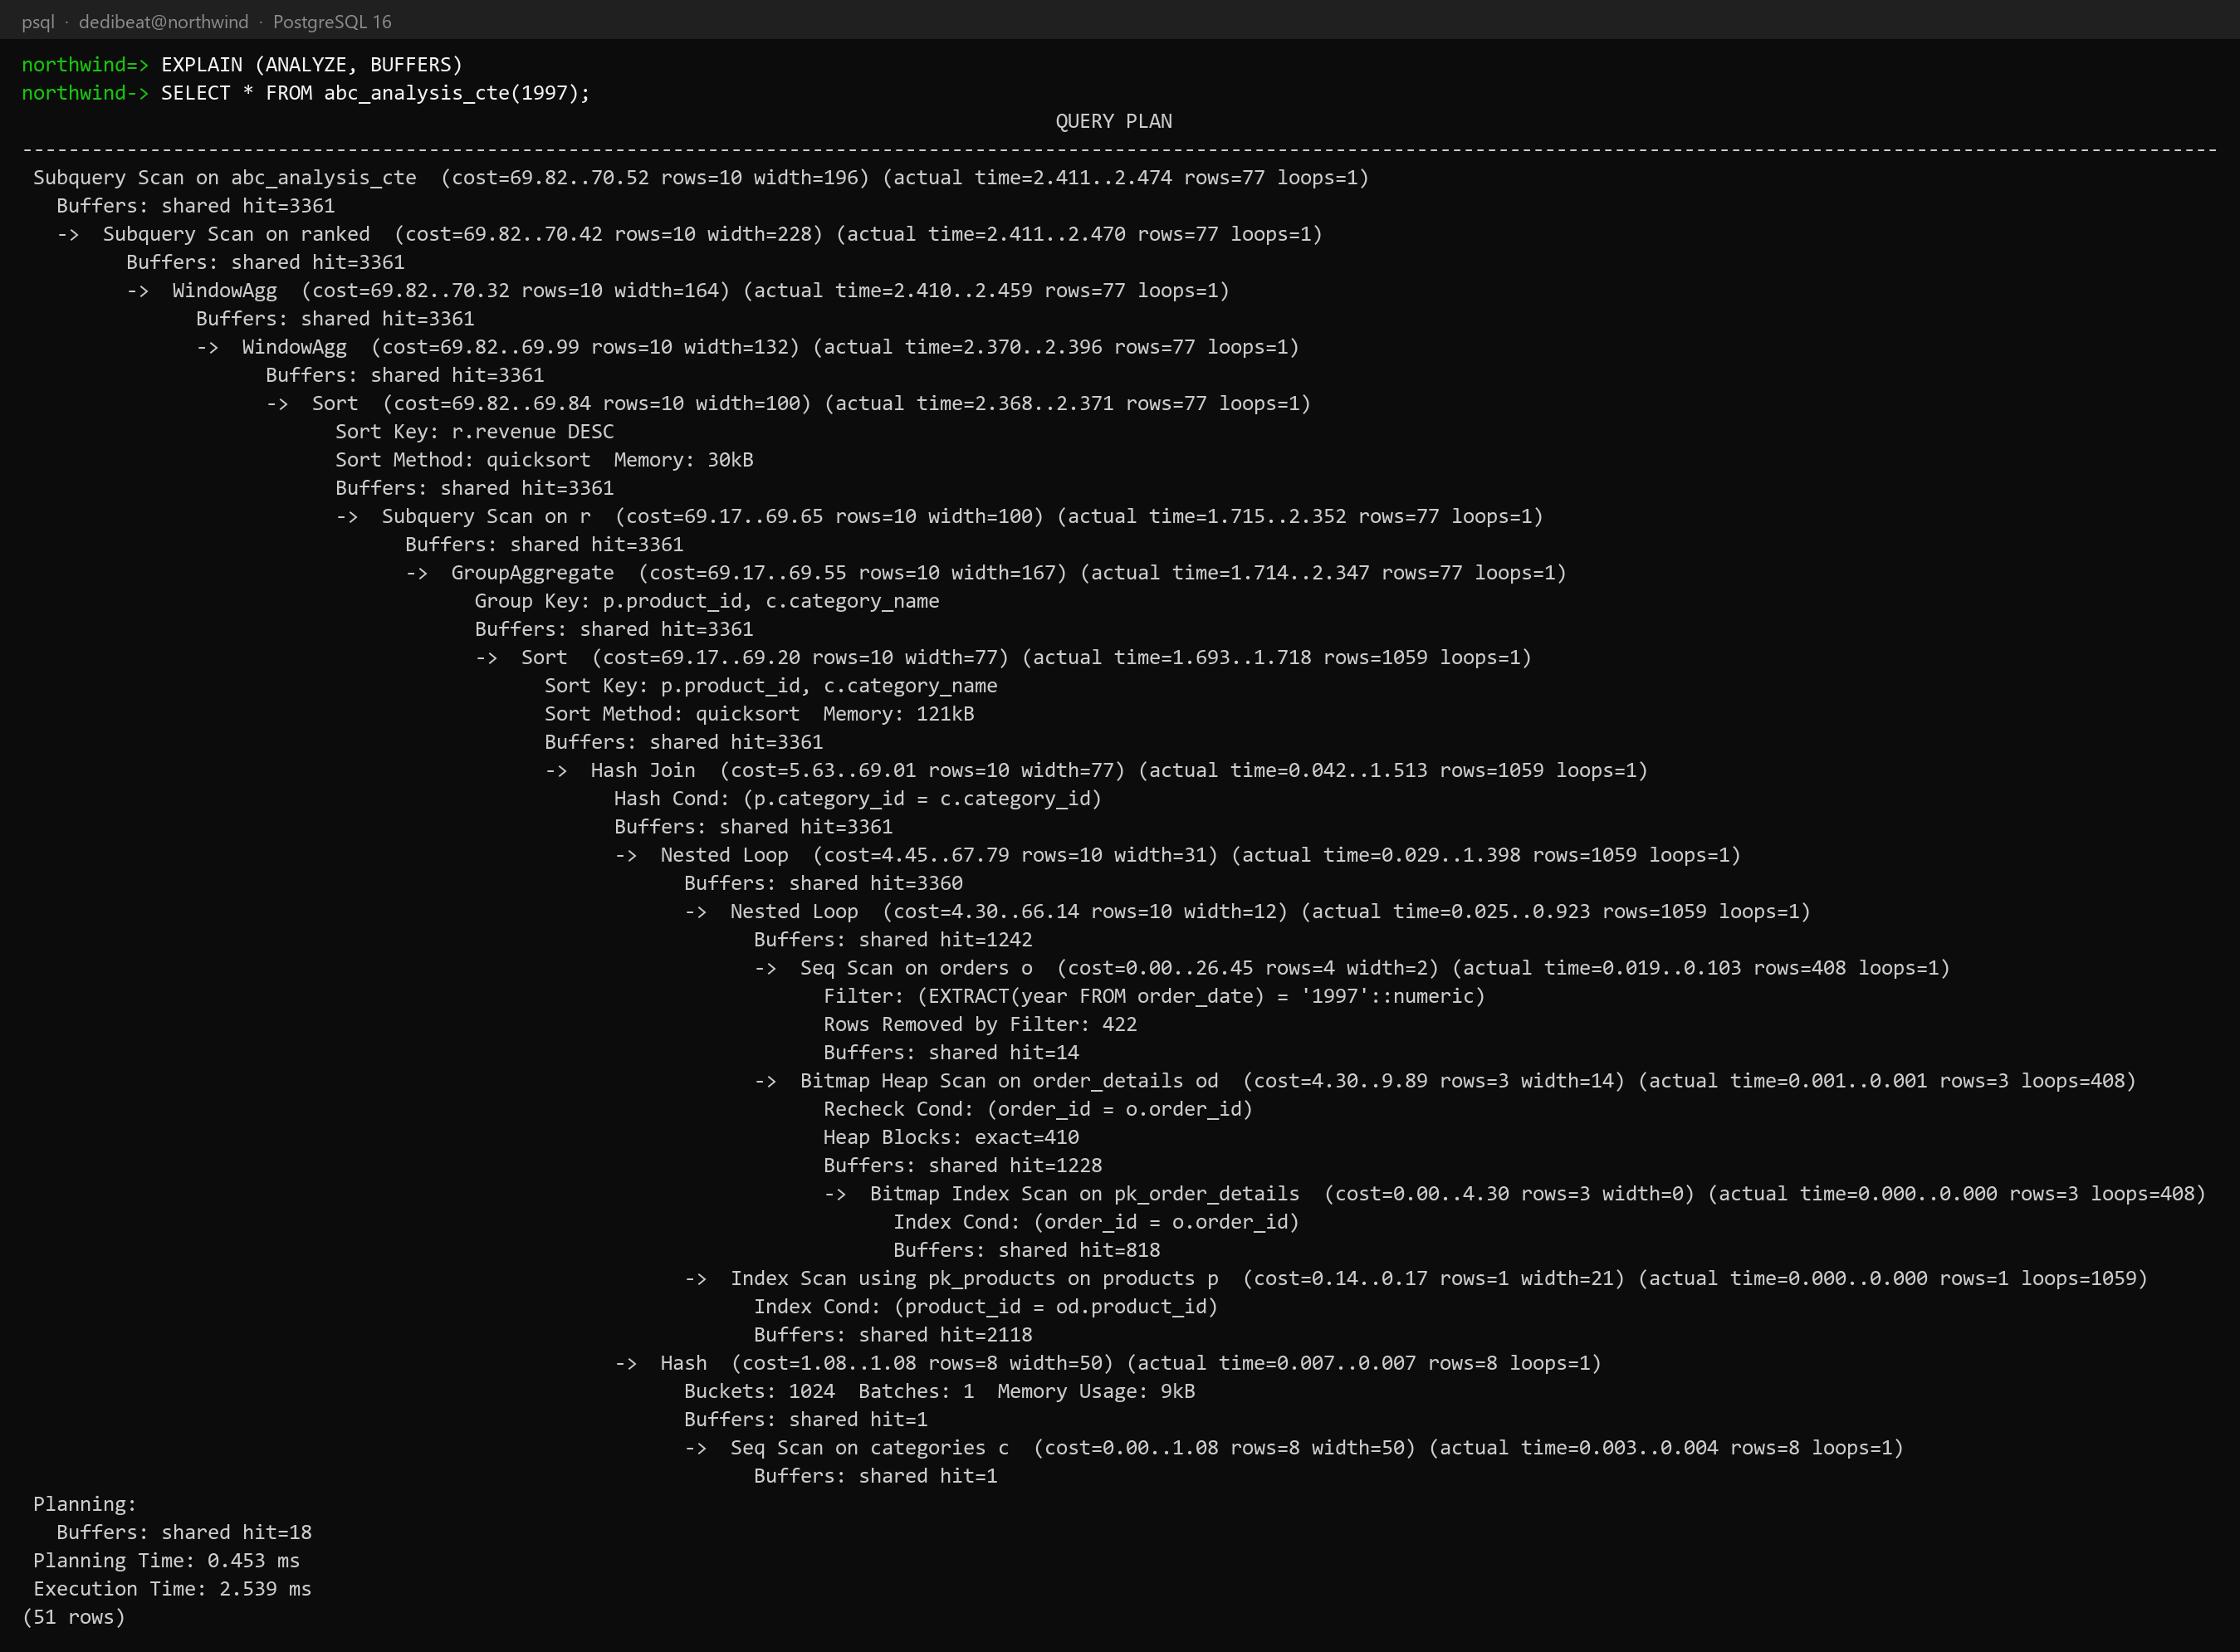
\includegraphics[angle=90,width=\textwidth]{img/ex10e.png}
  \par\vspace{4pt}
  {\small\color{captiongray}Зураг 10.6: CTE хувилбарын бүрэн төлөвлөгөө (\id{psql}). SQL функц inline хийгдсэн тул бүх зангилаа харагдана.\par}
\end{center}

\end{document}
